	\subsection{Les différentes familles de diagrammes}
Nous pouvons regrouper les diagrammes en différentes familles. Néanmoins, les frontières de ces dernières ne sont pas totalement étanches. Il se peut que certains diagrammes aient des caractéristiques de plusieurs familles à la fois. Les diagrammes mathématiques servent à représenter des concepts géométriques ou arithmétiques par l'usage spécifique d'idiomes, de lignes, de cercles et d'étiquettes alphabétiques. Ils servent par exemple à calculer la position d'une planète ou d'une étoile. Les diagrammes astrologiques montrent la position des astres à un moment donné pour en tirer des prédictions ou des interprétations sur les activités humaines. Ils sont dessinés à l'aide de lignes, de cercles et d'un langage graphique. Les diagrammes d'instrument permettent de comprendre le fonctionnement ou la structure d'un instrument astronomique comme l'astrolabe ou le quadrant afin de réaliser une observation ou un calcul. Ils sont représentés à l'aide de graduations, de nombres, de lignes et de cercles plus métriques que dans les autres familles. Pour finir, le diagramme cosmologique montre l'organisation de l'univers dans son ensemble par le biais de l'utilisation d'un langage de couleur et de texture\footcite{Conference2025Long2025}.


\subsection{Construire le stemma codicum de l'œuvre à partir des diagrammes}

En 2014, Dominique Raynaud publie un article nommé \textit{"Building the stemma codicum from geometric diagrams. A treatise on optics by Ibn al-Haytham as a test case"} dans lequel il expose une idée novatrice : il veut établir le \textit{stemma codicum} d'une tradition écrite uniquement à partir de diagrammes\footcite{raynaudBuildingStemmaCodicum2014}.

Un \textit{stemma codicum} est une représentation de toutes les étapes de la transmission d'une œuvre sous la forme d'un arbre inversé en établissant des relations entre les différents manuscrits. Le but de l'éditeur est alors de reconstituer le texte le plus proche du manuscrit original perdu que l'on nomme \og archétype \fg. Lorsqu'un texte est copié à plusieurs reprises, il constitue une \og tradition littéraire \fg dont les exemplaires sont nommés \og témoins \fg dans le domaine de la philologie. Pour tenter de reconstituer le \textit{stemma codicum} il est donc nécessaire de relever les différentes variantes provenant des divers manuscrits\footcite{pouliquenUsingLatticesReconstructing}.

Pour établir un \textit{stemma codicum} à partir de diagrammes, Dominique Raynaud emprunte à la biologie le principe de cladistique. Il s'agit \og d'une méthode de classification biologique qui exprime la phylogénie, c'est à dire les relations de parenté existant entre les êtres vivants \fg. Cette méthode \og repose sur le partage de caractères hérités d'une ascendance commune \fg, c'est-à-dire d'un \og ancêtre commun \fg \footcite{tassyCLADISTIQUE2012}.

Il explique que pour étudier les différents témoins d'une œuvre et les traditions qui l'entourent, il faut se baser sur les erreurs afin de réaliser un arbre généalogique. Nous pouvons affirmer qu'en utilisant cette démarche, il choisit de suivre la méthode de Lachmann. Il s'agit d'une méthode philologique élaborée au XIXe siècle par le philologue allemand Karl Lachmann dite de l'erreur commune. Ce dernier défendait la thèse suivante : Si un des témoins du texte présente une erreur, alors il y a de fortes chances que cette erreur soit aussi présente dans son descendant\footcite{pouliquenUsingLatticesReconstructing}.

Dominique Raynaud teste sa méthode sur un traité d'optique d'Ibn al-Haytham. En suivant cette démarche, il est arrivé à constituer le premier \textit{stemma} de diagrammes jamais publié. Ce dernier a été réalisé à partir des cinq témoins contenant l'œuvre : 


\begin{figure}[h]
	\centering
	\begin{subfigure}{0.48\linewidth}
		\centering
		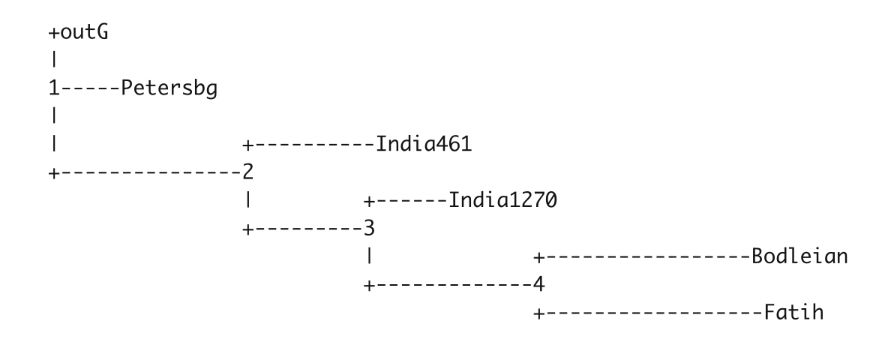
\includegraphics[width=\linewidth]{images/diagram_stemma.png}
	\end{subfigure}
	\hfill
	\begin{subfigure}{0.48\linewidth}
		\centering
		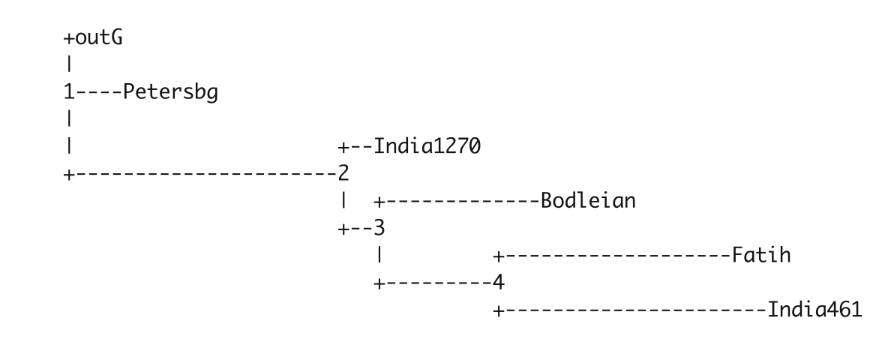
\includegraphics[width=\linewidth]{images/text_stemma.png}
	\end{subfigure}
	\caption{Stemmata pour les diagrammes (à gauche) et pour le texte (à droite) \footcite{raynaudBuildingStemmaCodicum2014}}
	\label{fig:stemma}
\end{figure}


En y regardant plus en détail, nous pouvons voir qu'il y a une forte similitude entre le \textit{stemma} textuel et le \textit{stemma} des diagrammes. Il en vient à la conclusion suivante : Quand les diagrammes sont intégrés au texte, il est envisageable de ne faire qu'un seul arbre pour les deux. Néanmoins, si les diagrammes ont été copiés a posteriori du texte ou qu'ils ont été corrigés par la suite, mieux vaut réaliser deux \textit{stemmata} distincts et étudier leur transmissions séparément. Le fait qu'ils aient été copiés par des personnes différentes à des moments différents impacte fortement leur étude. Il est même plus avantageux de réaliser le \textit{stemma codicum} d'une tradition mathématique à partir des diagrammes. La densité d'erreur serait sept à huit fois plus élevée dans un diagramme géométrique que dans un texte occupant la même superficie. Dans la mesure où sa méthode repose sur le relevé d'erreurs, il est plus judicieux de réaliser un \textit{stemma} avec des diagrammes\footcite{raynaudBuildingStemmaCodicum2014}.

Il nous est possible de retracer l'historique d'une œuvre grâce aux diagrammes. Cependant, ces derniers sont des éléments iconographiques complexes et il convient de les étudier de manière rigoureuse.